\documentclass[]{dukedissertation}
%\documentclass[economy,twoside,bind]{dukedissertation}
% Use the second for a single-spaced copy suitable for duplex printing
% and binding.

% Other useful options (there are more options documented in Chapter 2):
%  * draft -- don't actually include images, print a black bar on overful
%             hboxes
%  * MS    -- Format for a Master's Thesis.  No UMI abstract page, some 
%             textual changes to title page.  


% Useful packages for dissertation writing:
\usepackage{amsmath, amssymb, amsfonts, amsthm}
\usepackage{graphicx}
\usepackage{natbib}
\usepackage{color}
\usepackage{bm}
\usepackage{subfigure}
\usepackage{graphicx}
\usepackage{mathabx}
\usepackage{multirow}
\usepackage{setspace}
% \usepackage{cite}  % If you include this, hyperlink cites will
                     % break.  It's nice to use this package if your bibstyle
							% sorts entries by order-of-use, rather than
							% alphabetically (as plain does).
							
%Theorem, Lemma, etc. environments
\newtheorem{theorem}{Theorem}%[section]
\newtheorem{lemma}[theorem]{Lemma}
\newtheorem{proposition}[theorem]{Proposition}
\newtheorem{corollary}[theorem]{Corollary}
\newtheorem{result}[theorem]{Result}

% Personal commands and abbreviations.
%Define and personal commands here

%Graphics Path to find your pictures
\graphicspath{{./Pictures/}{../figure/}}


%-----------------------------------------------------------------------------%
% PREAMBLE 
%-----------------------------------------------------------------------------%
\author{[Anh Le]}
\title{[Two-Sided Matching Model]}
\supervisor{[Michael Ward]}
\department{[Department of Political Science]} % Appears as Department of \department
% Declare dissertation subject used on UMI abstract page.  List of
% categories: http://dissertations.umi.com/duke/subject_categories.html
%\subject{[Your Subject Here]}

\date{2018} % Anything but the year is ignored.

% Copyright text.  If undefined, default is 'All rights reserved'
% (Example sets the text to a hyperlinked Creative Commons Licence)
\copyrighttext{ All rights reserved except the rights granted by the\\
   \href{http://creativecommons.org/licenses/by-nc/3.0/us/}
        {Creative Commons Attribution-Noncommercial Licence}
}

% Committee Members other than supervisor.  No more than five beyond the
% supervisor allowed.
\member{[Eddy Malesky]}
\member{[Daniel Stegmueller]}
\member{[Peter Hoff]}
%-----------------------------------------------------------------------------%


%-----------------------------------------------------------------------------%
% HYPERREF: plain black hypertext references for ref's and cite's.
%-----------------------------------------------------------------------------%
\usepackage[pdftex, pdfusetitle, plainpages=false, 
				letterpaper, bookmarks, bookmarksnumbered,
				colorlinks, linkcolor=black, citecolor=black,
	         filecolor=black, urlcolor=black]
				{hyperref}

\begin{document}

%-----------------------------------------------------------------------------%
% TITLE PAGE -- provides UMI abstract title page & copyright if appropriate
%-----------------------------------------------------------------------------%
\maketitle

%-----------------------------------------------------------------------------%
% ABSTRACT -- included file should start with '\abstract'.
%-----------------------------------------------------------------------------%
%\abstract

While a Foreign Direct Investment (FDI) project can only materialize with the consent of both the multinational corporation (MNC) and the host country, the literature on FDI has focused only on the preference of MNCs. Through various case studies, I show that countries have varied and strategic preference, playing a substantial role in determining where FDI locates. Failing to recognize this two-sided matching nature of the FDI market, existing models of FDI produce wrong estimates of MNCs' preference. I introduce the two-sided matching model, investigate properties of the model, and apply it to study Japanese FDI in Southeast Asia. I show how to estimate the preference of both MNCs and countries for one another, modeling the two-sided matching process behind FDI location that scholars have always known but never been able to study quantitatively. With this model, scholars have a better understanding of what drives FDI location and policy makers can simulate FDI movement under hypothetical policy changes.}

%-----------------------------------------------------------------------------%
% DEDICATION -- OPTIONAL.  Put the text inside the braces.
%               (Long 'dedications' probably belong in the acknowledgements)
%-----------------------------------------------------------------------------%
%\dedication{If you want to dedicate your thesis to anyone do so here}

%-----------------------------------------------------------------------------%
% FRONTMATTER -- ToC is required, LoT and LoF are required if you have any
% tables or figures, respectively. List of Abbreviations and Symbols is 
% optional.
%-----------------------------------------------------------------------------%
\tableofcontents % Automatically generated
\listoftables	% If you have any tables, automatically generated
\listoffigures	% If you have any figures, automatically generated
%\abbreviations

% You can put here what you like, but here's an example
%Note the use of starred section commands here to produce proper division
%headers without bad '0.1' numbers or entries into the Table of Contents.
%Using the {\verb \begin{symbollist} } environment ensures that entries are
%properly spaced.

% \section*{Symbols}

% Put general notes about symbol usage in text here.  Notice this text is
% double-spaced, as required.

% \begin{symbollist}
% 	\item[$\mathbb{X}$] A blackboard bold $X$.  Neat.
% 	% Optional item argument makes the symbol/abbr
% 	\item[$\mathcal{X}$] A caligraphic $X$.  Neat.
% 	\item[$\mathfrak{X}$] A fraktur $X$.  Neat.
% 	\item[$\mathbf{X}$] A boldface $X$.
% 	\item[$\mathsf{X}$] A sans-serif $X$. Bad notation.
% 	\item[$\mathrm{X}$] A roman $X$.
% \end{symbollist}

\section*{Abbreviations}

\begin{symbollist}
  \item[AmCham] American Chamber of Commerce
  \item[ASEAN] Association of Southeast Asian nations
  \item[DGP] Data generating process
  \item[EM] Expectation maximization
	\item[FDI] Foreign direct investment
  \item[IPA] Investment promotion agency
  \item[IPE] International political economy
  \item[LDA] Latent Dirichlet allocation
	\item[MCMC] Markov chain Monte Carlo
  \item[MH] Metropolis-Hastings
	\item[MLE] Maximum likelihood estimation
  \item[MNC] Multinational corporation
  \item[MVN] Multivariate normal
  \item[SOE] State-owned enterprise
  \item[UNCTAD] United Nations Conference on Trade and Development
\end{symbollist}
} % List of Abbreviations. Start file with '\abbreviations'

%-----------------------------------------------------------------------------%
% ACKNOWLEDGEMENTS -- included file should start with '\acknowledgements'
%-----------------------------------------------------------------------------%
%\acknowledgements

I would like to thank my two advisors, Professor Edmund Malesky and Professor
Michael Ward. Professor Malesky's work on foreign direct investment and the
political economy of Vietnam was a big inspiration and \textit{the} reason for my
pursuing a PhD (and choosing Duke!) in the first place. He has taught me many
lessons in designing research, communicating results, and, most importantly,
being a good person. Professor Ward's approach to empirical work was an
eye-opener, pushing me to grow in ways I could not envision before. He nurtured
Ward lab, a community of smart and supportive people that I benefit from
tremendously even to this day. I used to tell every prospective student about
the Ward lab, and I really wish I still could.

I also benefited tremendously from the advice of Professor Peter Hoff and Professor Daniel Stegmueller. Without your kind and patient help, I would not have been able to develop and implement the statistical model for this dissertation. Professor Hoff's ``A First Course in Bayesian Statistical Methods'' is worth its weight in gold.

My thanks also to Professor Michael Newton for discussing two-sided matching model with me out of nothing but generosity, Professor John Allen Logan for sharing his US labor data, and Professor Andrew Delios for sharing his Japanese foreign direct investment data.

Finally, I would like to thank my wife, Huyen Le, for being there. (She did a lot more, but being there was already enough.)

%%% Local Variables:
%%% mode: latex
%%% TeX-master: "../AnhLe_dissertation.tex"
%%% End:}

%==============================================================================
%-----------------------------------------------------------------------------%
%
% MAIN BODY OF PAPER
%
%
%-----------------------------------------------------------------------------%
\chapter{Introduction}
\label{chap:introduction}

The global flow of Foreign Direct Investment (FDI) has risen from almost nothing
in the 1970s to over \$2.3 trillion dollars in 2016, becoming an important
source of global capital (Figure~\ref{fig:globalfdi}). For developing countries
especially, capital from multinational corporations (MNCs) is robust to global
economic downturns, prompting major international organizations to endorse FDI
as a key factor to economic development and poverty reduction
\citep{Mallampally1999, WorldEconomicForum2013}.\footnote{Indeed, while FDI into
  developed economies dropped almost 50\% during the 2000 recession and the 2008
  financial crisis, FDI into developing countries only experienced a plateau or
  a small reduction. More recently, as global FDI flow slipped in 2016 and 2017,
  FDI into developing countries still remained stable \citep{UNCTAD2018}.} Within the scholarly
field of International Political Economy (IPE), much of the literature starts
with the view that countries will always seek FDI for its various benefits
\citep{Jensen2008b}. Works in IPE tend to focus on \textit{how} countries can
attract FDI, and do not question \textit{whether} they want to do so
\citep{Jensen2003, Li2003, Li2006, Ahlquist2006}.\footnote{Two recent exceptions
  are \citet{Pinto2013, Pandya2016}, who are the first to examine variation in
  countries' demand for FDI.}

\begin{figure}[tbp]
  \centering
  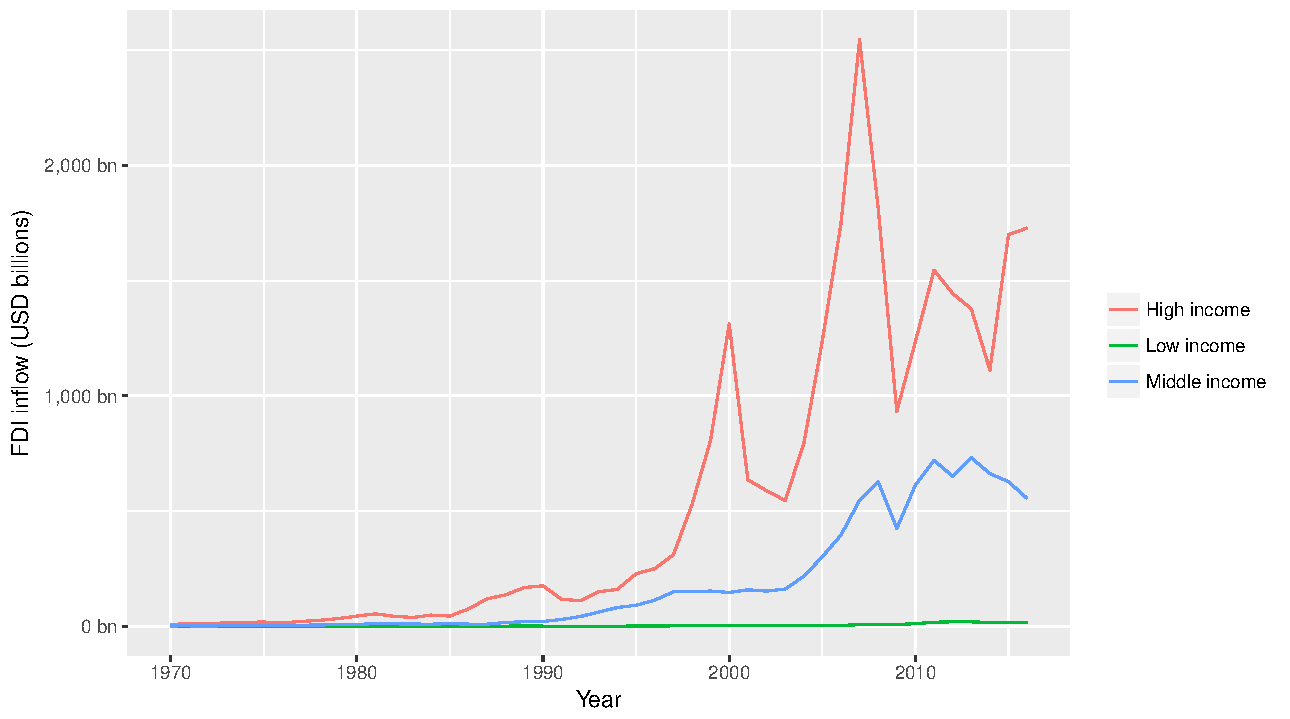
\includegraphics[width=0.8\textwidth,keepaspectratio]{../figure/global_fdi}
  \caption[FDI global inflow, 1970-2006.]{FDI global inflow, 1970-2006. The last
    four decades witness the growth of FDI into the most important source of
    global capital. Source: World Bank's World Development Indicators.}
  \label{fig:globalfdi}
\end{figure}

At first glance, the benefits of FDI seem obvious. FDI brings capital, create
jobs, contribute tax revenue, and promise technological spillover to the local
economy. Consider the impact of a high-tech facility by Intel on Vietnam's
economy. In 2006, Intel announced Saigon Hi-tech Park in Ho Chi Minh City,
Vietnam as the site for its largest chip testing and assembly in the world.
Starting from the initial plan of a US\$300 million facility, Intel decided
eight months later to increase the investment to US\$1 billion dollar, making up
almost 10\% of Vietnam's registered FDI in 2006. In 2016, Intel Products Vietnam
(IPV) employed 4000 workers at full capacity, exported US\$3.45 billion worth of
goods (18.2\% of Vietnam's electronics export), and contributes more than
US\$100 million to Vietnam's GDP in tax payment, salary, and profit. More
importantly, IPV also helped Vietnam address the skill shortage in engineering
and management. In the beginning, IPV hired workers earlier and trained them at
other Intel facilities in Asia. In the longer term, IPV developed an engineering
education program in partnership with Arizona State University and local
universities, training thousands of young Vietnamese engineers and giving them a
job. As a result, IPV's workers are vastly more productive: while IPV's
workforce only constituted 5\% of all workers at the Saigon Hi-tech Park, its
export value amounted to 72\%. Finally, Intel's decision to choose Ho Chi Minh
City over other candidate sites, including Chennai (India), Bangkok (Thailand),
and Dalian (China), was a significant marketing boost to Vietnam's image as a
destination capable of high-tech manufacturing. Following Intel, many other MNCs
opened high-tech facilities in Vietnam, including Samsung's three factories (in
2009, 2013, and 2014), Nokia/Microsoft (2012), and LG (2013) \citep{Dinh2016,
  UNCTAD2008}.

From a theoretical perspective, \citet{Findlay1978} argues that FDI plays a key
role in economic growth by upgrading the local economy's technological capability. As
well-known from neoclassical growth theory, diminishing returns to capital will
at one point stop capital from accumulating further, preventing long-run
economic growth from being driven by capital accumulation alone
\citep{Solow1956}. FDI can counteract this dynamic by helping local workers and
suppliers upgrade their productivity, either via training or demonstration.
In other words, technological spillover from FDI shifts the domestic factor-price
frontier to the right, resulting in a continually increasing capital stock and
sustained economic growth.

However, despite the theoretical arguments and shining examples such as Intel in
Vietnam, cross-country studies shows that
not all FDI are the same and that its effects are highly conditional. For
example, there is no conclusive evidence of FDI inflow having a positive effect on
growth \citep{Nair-Reichert2001, Carkovic2002} or poverty reduction
\citep{Guerra2009}. This puzzle opens a substantial literature on how the
growth-enhancing and spillover effect of FDI is conditional on the absorptive
capacity of the host economies, i.e. its level of human capital, technological
sophistication, and financial market development \citep{Durham2004,
  Nunnenkamp2004, Fu2008, Willem2004}. In addition, while the capital brought
and jobs created by FDI may be unconditionally good for the overall economy, its
distributional effects cut across constituencies in the host economy, creating
political cleavage across both sectoral and geographical divides
\citep{Chintrakarn2012, Goldberg2007, Nunnenkamp2007}.

Given the evidence on the conditional effect of FDI, it is no longer tenable to
assume that countries' preference for FDI is homogeneous. By holding this
assumption, we neglect the role of the state in shaping global capital flow,
falling prey to the discredited ``race to the bottom'' thesis of globalization
\citep{Mosley2005}. Arguably, examining countries' preference for FDI should be
of more interest to political scientists than the current focus on determinants
of MNCs' location, which often amounts to adding a political variable to an
existing economic model of FDI flow. In addition, even if we only care about
MNCs' preference, to get an accurate estimate we must still take into account
countries' preference. For example, consider the received wisdom that
democracies receive more FDI \citep{Jensen2008a}. Without controlling for
countries' preferences, it is difficult to interpret this finding as democracies
actively pursuing MNCs or as MNCs finding democracies attractive.

\section{Goal of the research}

My research aims to estimate the preference of countries and MNCs for each
other. I develop an empirical strategy that takes into account the two-sided
nature of the FDI market, i.e. a subsidiary can only materialize if both the MNC
and the host government agree. Recognizing that this two-sided matching dynamics
can also be found in the labor or the marriage markets, I adapt the statistical
models first developed in Sociology for labor and marriage markets and apply
them to the study of FDI \citep{Logan1996, Logan2008}.

In doing so, I simultaneously address three long-standing issues in the FDI
literature. First, I ``bring the state back in,'' filling the gap in the literature on the
variation of countries' preference for FDI.\footnote{\citet{Evans1985}'s
book argues that states are weighty actors with their own capabilities and
initiatives rather than an arena for societal and interest groups to negotiate
for their share. Here, I argue that states are weighty actors with their own
preferences rather than goods that MNCs pick and choose.} Two notable exceptions are
\citet{Pinto2013} and \citet{Pandya2016}, whose pioneering works propose
partisan politics and regime types as factors shaping preferences for FDI.
However, while their theories are ground-breaking, the empirical estimation of
countries' preference remains inadequate. In addition, these researchers have
not used their findings to re-estimate the preference of MNCs and disentangle
the ``push'' and ``pull'' factors of FDI flow.\footnote{``Push factors'' refer
  to characteristics of the home country and of the MNC, pushing capital out
  from its origin. ``Pull factors'' refer to the characteristics of the host
  country, pulling capital towards its destination.} Using a two-sided matching
model, I will naturally be able to estimate both sides' preference.

Second, I propose that we need to pay more attention to countries' preference
for different types of FDI. While the IPE literature has largely focused on the
quantity of FDI flow, countries pay much attention to the its type, using
various incentives and restrictions to target certain types of FDI. Indeed, MNCs
come with varying amount of capital, labor demand, and technological
sophistication, all of which have different effects on the host country's
economy. Just as the two-sided matching model can estimate MNCs' utility
function for countries' characteristics (e.g. market size, level of
development), it can also estimate countries' utility function for MNCs'
characteristics (e.g. technological sophistication, export strategy).

Third, while the majority of the literature uses FDI flow data, these data
are accounting constructs created to keep track of countries' balance of payment
and thus map poorly to concepts in Political Science theories. Very often, the
variable of interest in our theories is the scale of MNCs' activities in the
host country, which can be very different from the amount of border-crossing
capital thanks to MNCs' complex financial and tax strategies \citep{Kerner2014}.
Therefore, we would do much better testing our theories with firm-level
operational data. Because the two-sided matching model is a behavioral model in
which each actor's decision is a unit of observation, and we can naturally use
it to analyze firm-level data.

These three issues are related and represent the status quo in the FDI
literature. Data limitation forces scholars to look at country-level aggregate
FDI flow, making it difficult to study countries' preference for FDI types. And
without studying countries' preference, our current models of MNCs' location
choice are also suspect.

In sum, my dissertation benefits the field by using firm-level data to estimate
both firms' and countries' preference for each other's characteristics. In this
two-sided matching model, MNCs and countries evaluate their available options
according to their utility functions, choose the best alternative, culminating
in an MNC's subsidiary located in a host country.

Estimating this model would be straightforward if we observed not only
subsidiaries' locations but also their set of options (called their
``opportunity set'' in the matching literature).\footnote{Discrete choice models
  can be used to estimate the utility function when both the choice and the set
  of options are observed. Indeed, discrete choice models remain the dominant
  empirical approach in the industrial location literature, effectively ignoring
  the fact that not all MNCs have the same set of location options
  \citep{Arauzo-Carod2010}.} Unfortunately, while data on subsidiaries' location
are available, the opportunity set is generally unobserved as researchers cannot
peek into the negotiation process between countries and MNCs. The two-sided
matching model solves this problem by using the Metropolis-Hastings (MH)
algorithm, a Markov chain Monte Carlo (MCMC) approach that repeatedly samples
new opportunity sets and rejects them at an appropriate rate to approximate
their true distribution. In addition, the estimated preference parameters in the
two-sided model have a convenient interpretation as the relative weight of
different variables on MNCs' and countries' utility. This allows us to make
statements such as: ``In evaluating MNCs, China values a 2\% increase in the
firm's capital as much as a 1\% increase in labor demand.''

\section{Roadmap}

In the rest of this introductory chapter, I review in-depth the three issues in
the literature of FDI's political determinants, outlining the current attempts
to address them and how my approach can contribute to the solution.

In Chapter~\ref{chap:model}, I describe the two-sided matching model, including
both its game-theoretic origin and its statistical estimation.
Chapter~\ref{chap:simulation} uses simulations to demonstrate the correctness of
the model and explore its characteristics. Chapter~\ref{chap:labor} applies the
model on US labor market data, the original domain of the two-sided matching
approach, in order to compare with and expand upon previous results.
Chapter~\ref{chap:FDI} brings us back to the study of FDI, applying the model on
firm-level data of Japanese MNCs in East and Southeast Asia.
Chapter~\ref{chap:conclusion} concludes and explores potential applications of
the two-sided matching model in other areas of Political Science.

\section{Three issues in the FDI literature}
\label{sec:literature_issues}

\subsection{Estimating countries' demand for FDI}

The IPE literature on the political determinants of FDI has overwhelmingly
focused on what MNCs demand from countries, not what countries demand from MNCs.
In this literature, politics matters, but only in terms of what
political factors make countries attractive to MNCs. As Jensen states in
the introduction of \textit{Nation-states and the multinational corporation}:

\begin{quote}
  Which government policies prove beneficial to multinational corporations?
Which political institutions provide multinational corporations with credible
commitments to these market-friendly policies? These emerge as the central
questions of this book.
\end{quote}

Other scholars share the same line of inquiry \citep{Ahlquist2006, Busse2007,
  Buthe2008, Li2003}. In their theoretical argument, the central dynamics of the
negotiation between countries and MNCs is that FDI is mobile before MNCs make
the investment on the ground but immobile after. Since the cost of relocation is
higher the more investment MNCs commit, the original bargain between the host
country and the MNC become increasingly obsolete as the host country can alter
the original bargain at the expense of the MNC, knowing that relocating would
cost the MNC dearly. Therefore, certain political
institutions, such as democracy, veto players, and federalism, increase FDI
inflow because they can credibly commit not to change their policies \textit{ex
  post}, and are thus
attractive to MNCs.

Cost of doing business arguments. 

In theorizing FDI inflow largely as a function of MNCs' preference, the FDI
literature implicitly assumes that countries are eager to receive as much FDI as
possible. The two common empirical approaches in the literature expose this
assumption. In the first approach, researchers build a regression model with FDI
inflow as the dependent variable and a political factor as the independent
variable of interest. The problem with this model is that it is impossible to
interpret the political factor as an attraction to MNC or as a motivator of
countries' demand for FDI. Consider \citet{Jensen2005}'s finding that federalism
is positively associated with FDI inflow. The authors interpret this correlation
as federalism constraining the whim of the central government, increasing policy
stabilities, and thus making the country attractive to MNCs. However, the
alternative explanation is that local governments in a decentralized system
compete more intensely for FDI, driving up the FDI inflow. For example, As China
decentralized in the late 1980s and early 1990s, local governments gained the
authority to approve foreign investment up to a certain size, thus able to court
MNCs without asking the central government for permission.\footnote{Similar to
  China's broader economic reform, decentralization in China's FDI policies
  happened incrementally. In 1979, China first allowed FDI in four Special
  Economic Zones, i.e. Shenzhen, Zhuhai, Shantou (near Hong Kong), and Xiamen
  (near Taiwan). As the economic benefits of FDI became clear, provinces started
  clamoring for the ability to attract FDI themselves. Therefore, in 1984, China
  allowed 14 coastal cities to approve FDI projects themselves, and in the early
  1990s, allowed inland regions to do the same. \citet{Gallagher2002, Shirk1993}
  discuss how the coalition for decentralization expanded over this period, and
  \citet{Coase2012} provides a historical account of China's economic reform
  more broadly.} In addition, local governments could keep all revenue in excess
of a quota pre-negotiated with the central government, further motivating them
to bring in MNCs as a lucrative source of tax revenue. Having both the authority
and the incentive to attract MNCs, Chinese local governments engaged in an
intense competition for MNCs. For example, while there were only 117 development
zones in 1991, the number exploded to 2700 in 1992, of which only 95 were
initiated by central ministries \citep{Montinola1995}. Far from
\citet{Jensen2005}'s argument, China's federalism did not increase FDI inflow by
producing a static policy environment that MNCs like. On the contrary,
federalism incentivized Chinese local governments to demand FDI, fostering
local policy experiments that were anything but stable.\footnote{A very similar
  account of decentralization causing provincial demand and competition for FDI happened in Vietnam
  as well \citep{Malesky2004c}.}

In the second approach, researchers estimate MNCs' preference using discrete
choice model. The dependent variable is the MNC's choice of a location over all
the others, and the independent variable of interest is a characteristic of the
location \citep{Arauzo-Carod2010}. In discrete choice model, the assumption is
that all locations are available for the MNC to pick and choose, effectively
ruling out the possibility that the host country can decline the MNC's
investment proposal. Such an assumption is unfounded. For example, in 2007, Da Nang, a
central province of Vietnam known for its public governance quality, turned down
\$2.5 billion dollars from
a Taiwanese-Japanese steel factory and a Japanese paper pulp factory for
environmental concern \citep{NLD}. In 2014, even in tough times, when Da Nang's and Vietnam's
FDI inflow was
merely half of the previous year, Da Nang's attitude towards FDI remained
selective, declining a \$200-million Hong Kong textile factory and a 30-hectare Korean dying
facility, showing its  

A historical and comparative examination of FDI policies makes it clear that the
assumption of countries' unequivocal demand for FDI is not true. First,
historically countries are not so open to FDI.

Second, there is substantial variation across countries.

Third, countries are very strategic in their FDI policies, changing it over
time to fit with the political and economic conditions of the countries.


We have made this mistake before. Despite earlier pessimism about countries engaging in a race to the bottom to
attract footloose global capital, empirical evidence shows that countries'
policies still vary substantially \citep{Drezner2001}. While the broader IPE
literature has recognized the variation in countries' trade, welfare,
environmental, and fiscal policies in the face of globalization, we have
surprisingly done less work to explain variation in countries' demand for FDI.
Neglecting countries' demand for FDI is both a theoretical and an empirical gap
in our FDI literature. Theoretically, much of the literature on the political
determinants of FDI only examines how the political factors are assessed by the MNC, assume that countries want as much FDI as possible and the
only problem is that they cannot credibly commit to reduce the uncertainty in
order to attract business. On the empirical side, in using discrete choice model
to model MNCs' location decision, the literature assumes that all MNCs have
access to all locations.

Recognizing this gap in the literature, \citet{Pinto2013} and \citet{Pandya2016}
recently broke ground in this area. Similar to the rich IPE literature in
international trade, these studies argue that countries' demand for FDI varies
according to FDI's distributive effect on their domestic constituencies
\citep{Broz2001, Milner2005a}. In this theoretical framework, labor supports FDI
because foreign firms bring capital that increases the demand for labor and
raises productivity, both of which lead to higher wage. On the other hand,
domestic firms oppose FDI because foreign firms compete for local labor, inputs,
and markets. Both \citet{Pinto2013} and \citet{Pandya2016} formulate their
theories as a variant of this labor-vs-business tension, which surfaces in the
former work as left-vs-right governments, and in the latter as
democratic-vs-authoritarian regimes.

While these pioneering works have enriched our understanding of the relationship
between politics and FDI, their empirical approaches do not satisfactorily
measure countries' demand for FDI, leaving their theoretical arguments untested.

Consider \citet{Pinto2013}'s approach. The author controls for economic and
institutional factors that affect FDI flow into a country, then claims that
what's left in the residual is the country's demand for
FDI.\footnote{Specifically, the estimation of FDI openness involves two steps.
  First, the author runs a gravity model explaining bilateral FDI flows,
  estimating the intercept as the host country-year fixed effect. Second, this
  fixed effect is then regressed on several economic and endowment factors of
  that country-year (i.e. GDP, GDP per capita, average school years, arable
  land). The residual in the second stage is considered the country's ``FDI
  openness'' in that year.} For this approach to be valid, every economic,
institutional, and endowment factors that affect FDI flow has to be controlled
for, leaving only the country's demand in the error term. This claim is much
stronger than the common assumption of exogenous error, which is valid as long
as the omitted factors are uncorrelated with the independent variable of
interest. Framed substantively, since the residual is likely to contain more
than just the country's demand for FDI, if we observe an abnormally high level
of FDI, we do not know whether it is because the country welcomes FDI or because
MNCs find something attractive in the country.\footnote{In addition, this
  approach requires data on bilateral FDI flow, ideally disaggregated by
  sectors. Therefore, this approach is limited to OECD countries only
  \citep{Pinto2008}. During the period the authors study, 1980-2000, OECD
  countries account for 95\% of global FDI outflow and 90\% of inflow. However,
  since then the role of the developed world in global FDI has declined sharply,
  reducing to 60.8\% of outflow and 40.6\% of inflow in 2014
  \citep{UNCTAD2015}.}

In contrast to \citet{Pinto2013}'s statistical approach, \citet{Pandya2014,
  Pandya2016} attempts to find a proxy for countries' demand for FDI. The author
uses the annual US Investment Climate Reports to construct the number of
industries that have foreign ownership restrictions or face investment
screening. The advantages of this measurement are its ease of interpretation and
its availability for many countries. However, two problems remain. First, adding
up the raw count of restricted industries is not appropriate because industries
are not the same. For example, given the reach of the banking sector into all
corners of the economy, a country's opening up its financial industry indicates
much more FDI-friendliness than, say, allowing foreign furniture makers to set
up shops. Since the theoretical argument is driven by FDI's distributive effect,
we must not ignore the varying impact of FDI across sectoral constituencies.

Second, according to the coding rule, an industry is coded as free if there is
no mention of restriction. However, when there is little FDI, US Investment
Climate Report may find it not worth mentioning and does not report the
restrictions. Therefore, ``zero restriction'' in the dataset can either mean
that a country is very closed or very open to FDI. This concern is not
hypothetical. Figure \ref{fig:china_fdi_restriction} shows that, following the
coding of the US Investment Climate Reports, China seemed 100\% open to FDI up
until 1986 when it started imposing restrictions. The reality is the opposite.
Prior to 1986, only limited FDI was allowed as joint-venture in Special Economic
Zones (SEZ). The year of 1986 was, in fact, the first time China allowed any
wholly owned FDI outside of SEZs.

\begin{figure}[tbp] \centering
  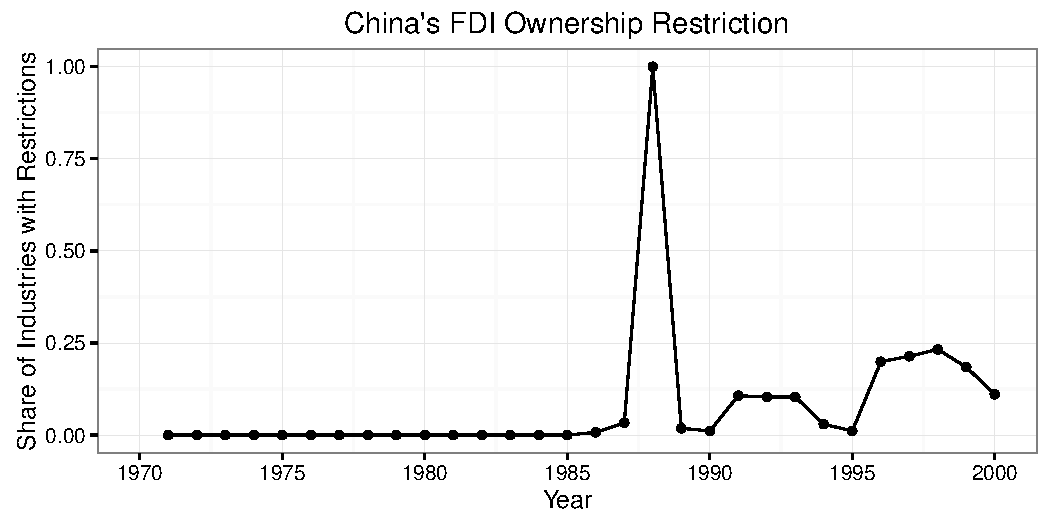
\includegraphics[width=0.8\textwidth,keepaspectratio]{china_fdi_restriction}
  \caption[China's FDI ownership restriction.]{China's FDI ownership
    restriction, as coded in \citet{Pandya2010}. Prior to 1986, FDI in China was
    limited to few experimental Special Economic Zones, and thus not mentioned
    in US Investment Reports. The sharp spike in 1988 also does not seem to
    correspond to any actual change in policy, and likely another artifact of
    reporting. (See \citet{Zebregs2002} for a historical overview of China's FDI
    policy.)}
  \label{fig:china_fdi_restriction}
\end{figure}

The two-sided matching model circumvents these thorny measurement issues by
modeling countries' demand for FDI directly. Intuitively, if we observe that a
country welcomes certain firms to invest but not others, we can compare the
characteristics of the invited and the uninvited firms to infer that country's
preference for FDI.

\subsection{Estimating countries' preference for types of FDI}

In addition to estimating countries' demand for FDI, we should also examine
countries' preference for different types of FDI. Indeed, while the Political
Science literature has focused almost exclusively on the quantity of FDI,
treating all FDI as one homogeneous flow of capital, policy makers seem to pay
much more attention to distinguishing its types. Commenting on the role of
International Investment Agreements, \citet{UNCTAD2015} says, ``Today,
increasing the quantity of investment is not enough. What matters is its
quality, i.e. the extent to which investment delivers concrete sustainable
development benefits.'' Governments in developing countries all offer various
forms of tax incentives and fee waivers to attract FDI that invests in a remote
region, brings new technology, or focuses on exporting \citep{Ricupero2000}. For
example, since 2006, China's official FDI policy has been ``quality over
quantity,'' promoting FDI with intense R\&D in high-productivity sectors
\citep{Guangzhou2011}.

Despite the importance of disaggregating FDI by its type, two data limitations
prevent researchers from doing so. First, FDI flow data typically does not
disaggregate into types of FDI. \citet{Alfaro2007} attempt to get around this
problem by using Germany's sectoral skill intensity as the proxy for the FDI
quality from each sector in the OECD. To do so is to assume that 1) Germany's
sectoral variation is the same as everyone else's in the OECD, and 2) there is
little variation in skill intensity within a sector. Both assumptions are
untenable, especially since the authors divide all manufacturing industries into
only two categories: low skill and high skill.

Second, even if we can differentiate types of FDI, it remains an open question
how to estimate countries' preference for them. \citet{Alfaro2007} use
information from IPAs' website and survey response as a proxy for their
countries' preference---if an IPA lists an industry as a ``target industry,''
the authors say that the country wants to attract that type of FDI. While this
approach seems reasonable at first glance,
Figure~\ref{fig:IPA_target_industries} shows that there is little variation in
what IPAs claim to be their target industries. Because investment promotion is
mainly a marketing and aspirational exercise, almost everyone claims that they
target manufacturing, advanced manufacturing, and infrastructure. In addition,
if we use IPAs as a proxy for countries' preferences, we should also model the
selection process in which the countries that decide to establish an IPA may not
be the same as those who do not. Both of these issues are not addressed by
\citet{Alfaro2007}, and we are still in need of a way to estimate countries'
preference for different types of FDI.

\begin{figure}[tbp] \centering
  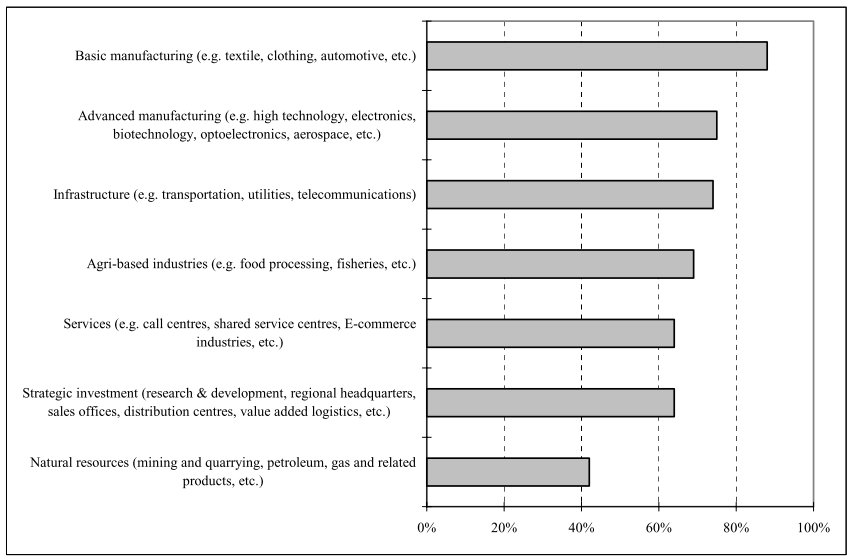
\includegraphics[width=\textwidth,keepaspectratio]{../figure/IPA_target_industries}
  \caption[Target industries by IPA around the world.]{Target industries by IPAs
    around the world. Because of the image building aspect of investment
    promotion, almost all IPAs say that they want to attract ``manufacturing,''
    ``advanced manufacturing,'' and ``infrastructure.'' Therefore, using what is
    listed as investment priorities may not be a reliable way to measure
    countries' preference for FDI. Source: \citet{UNCTAD2001}}
  \label{fig:IPA_target_industries}
\end{figure}

In sum, differentiating FDI by sectors only gives us a crude typology of FDI. We
can address this challenge using firm-level data, giving us information on not
only a firm's sector but also its operational characteristics, such as research
and development (R\&D) expenditure or export intensity. These measures are
firm-specific and get closer to what countries are looking for in FDI projects.
Using R\&D expenditure or export intensity as firms' characteristics in the
two-sided matching model, I will be able to estimate countries' preferences for
these traits.

\subsection{Measuring MNCs' activities}

As \citet{Kerner2014} argues, the IPE literature on FDI is a bit of a misnomer.
Political scientists are rarely interested in FDI \textit{per se}---rather, they
are interested in the activities of MNCs, which in turn, affect other important
issues such as nation-state autonomy \citep{Mosley2005}, economic development
\citep{Moran1998}, labor standards \citep{Mosley2007}, and environmental
policies \citep{Prakash2007}. However, while the theory involves MNCs as the
central actor in the causal mechanism, the empirics often uses FDI flow as the
variable of interest. These two concepts---the level of MNCs' affiliate
activities in a country and FDI inflow into a country---are not the same.

Consider the definition of FDI from UNCTAD, the main producer of FDI data widely
used by researchers:

\begin{quote} FDI has three components: equity capital, reinvested earnings and
  intra-company loans.
  \begin{itemize}
  \item Equity capital, i.e. the foreign investor’s purchase of shares of an
    enterprise [in the host country].
  \item Reinvested earnings, i.e. the foreign investor’s share \ldots of
    earnings not distributed as dividends by affiliates, or earnings not
    remitted to the foreign investor.
  \item Intra-company loans between direct investors and affiliate enterprises.
  \end{itemize} \citep[245]{UNCTAD2007}
\end{quote}

In essence, FDI data captures the amount of capital that crosses border. It is a
poor proxy for the scale of MNCs' activities in the host country because it
overlooks important components of MNCs' activities while including components
that are only relevant for balance of payment statistics
\citep{Beugelsdijk2010}.

Consider the argument that FDI is the driver for the diffusion of labor
standards across countries. \citet{Mosley2007} theorizes that FDI can have this
effect through three channels. First, MNCs may pressure the host government for
better rule of law and social programs. For MNCs to be able to effectively exert
this pressure, they must prove themselves valuable to the government by
providing jobs or tax revenue. Both of these factors are tenuously related to
the amount of foreign capital inside the host country. Indeed, an MNC can employ
thousands of employees, pay millions in tax, but show up as a net 0 on FDI flow
data because the profit is repatriated to the foreign investor or through
intra-company loans.\footnote{The issue of intra-company loans is particularly
  fraught with issues because companies very frequently use intra-company loans
  to get out of paying tax in a country. These loans will be recorded on the
  book as a massive outflow, even though the MNC still has a large presence on
  the ground.} The scale of MNCs' operation is further understated because FDI
statistics does not take into account capital raised locally. Also not included
is the superior productivity of MNCs, which acts as an important multiplier when
translating the amount of capital to the amount of output.

Second, scholars argue that MNCs may bring along best practices for workers'
rights and spread it to local firms. If this spillover effect happens via
competition, i.e. MNCs providing better working condition and forcing local
firms to compete, then MNCs must employ a lot of labor for this effect to be
noticeable. Or if the spillover happens via demonstration, then MNCs must form a
lot of linkages with local firms, as suppliers and buyers, for the diffusion of
norms to happen. Both the size of the labor force and the type of linkages with
the local economy are not captured by FDI flow statistics.

Third, scholars argue that MNCs may care more about labor quality than its cost,
and thus may invest in higher wages, better benefits, or more training. Once
again, for this effect to be noticeable, the MNC's industry, size of labor
force, and investment in productivity all matter a lot more than how much
capital it brings in and out of the country. In addition, non-equity
transactions between the parent company and the subsidiary, such as transfer of
knowledge, technology, and management practices, are not counted in FDI flow
statistics, thus excluding another component that is arguably much more
important to labor quality than the amount of capital.\footnote{These issues are
  not isolated to studies of FDI and labor standards, but are common to the
  whole IPE literature of the effect of FDI on policy convergence, such as
  environmental policies \citep{Prakash2007}.}

This mismatch between theory and empirics may also be a reason behind the
unsettled debate on the effect of FDI on poverty reduction. Scholars have
theorized that FDI can lead to economic development through three channels:
cheaper goods, technology transfer, and tax revenue. Once again, the causal
variable in the second and third channels is the scale and the type of MNCs'
activities in the host country, not necessarily the amount of capital crossing
the border. Indeed, productivity spillover is highly conditional on the
technological capability of the MNC and whether it forms thick linkages with the
local suppliers. The effect of FDI via tax revenue is also fraught with issues,
as MNCs frequently use intra-company transactions to artificially reduce book
profit and get out of paying tax \citep{Malesky2015c}.\footnote{These tactics
  are called ``transfer pricing,'' and can include tactics such as charging for
  internal intellectual properties and services whose price can be set
  arbitrarily by the firm} Since FDI flow statistics do not record these
intra-company transactions, it is not surprising that researchers reach the
confusing conclusion that FDI does not generate tax revenue.

What about studies that use FDI as the dependent variable, and are thus perhaps
interested in the flow of capital in and of itself?\footnote{Arguably, political
  scientists are not interested in the flow of capital in and of itself, but
  because of its implications for development, state autonomy, and other effects
  on policy. The discussion above has shown how problematic it is to study these
  effect of FDI using FDI flow data.} The vast majority of these studies on the
determinants of FDI flow rely on the ``obsolescing bargain'' model. Originally
developed by \citet{Vernon1971}, the model is so named because the bargaining
dynamics between the MNC and the host government changes over time, initially
favoring the MNC and gradually tips towards the host government as the MNC
commits more fixed capital on the ground. Indeed, knowing that it is costly for
the MNC to uproot its increasingly large and immobile operation, the host
government can unilaterally alter the original bargain, most egregiously by
expropriating the MNC's asset and profit, but more often via ``creeping
expropriation,'' e.g. increased tax or tougher regulation \citep{Li2009a}.
Political economists argue that MNCs are acutely aware of the ``obsolescing
bargain,'' and thus prefer to invest in countries whose governments can make a
credible commitment that they will not alter the original deal. This argument
translates into a large literature claiming that MNCs prefer countries with
democratic accountability \citep{Jensen2003}, a federal system
\citep{Jensen2005}, membership in international trade agreements
\citep{Buthe2008}, less political risk \citep{Beazer2011, Graham2010}, or more
veto points \citep{Choi2008}.

The linchpin of this argument is the assumption that FDI capital is illiquid and
cannot be quickly removed from the host country at will. This assumption is not
fully warranted. According to the US Bureau of Economic Analysis (BEA)'s 2004
survey, 43\% of US MNCs' balance sheet comprises of liquid assets that can be
liquidated within one year under normal operating situations. Among the 57\% of
the balance sheet that are illiquid, 24\% are ``other non-current assets,''
which include non-tangible assets like brand names, trademarks, and
patents---some of which are not expected to be liquidated but can be easily
removed from host countries. Only another 24\% of the balance sheet is made up
of physical capital, i.e. Plant, Property, and Equipment (PPE), which cannot be
easily moved and match most closely to what we have in mind as the ``illiquid
capital'' in the obsolescing bargain model \citep[113]{Kerner2014a}. Since FDI
flow data does not distinguish between liquid and illiquid capital, it is
suspect to use FDI flow data to test the ``obsolescing bargain'' argument,
calling into questions the entire literature on the political determinants of
FDI.

Besides the conceptual mismatch between FDI flow and MNCs' activities, from a
statistical standpoint, this measurement error may also be a contributing factor
to why there is little consensus in the FDI literature. Even if the measurement
error is random, it will inflate the standard error of our estimate when FDI is
the dependent variable, and bias our estimate towards 0 when FDI is the
independent variable. These effects may explain \citet{Jensen2012}'s surprising
finding that lower corporate tax rate does not lead to more FDI flow, or the
mixed empirical evidence for the relationship between FDI and development
\citep[108]{Mold2004}.

Even more worryingly, the measurement error is unlikely to be
random.\footnote{See \citet{Gallop2017} for a recent and more comprehensive
  discussion of measurement error in political science research.} For example,
the amount of locally raised capital---an important source of capital for MNCs
yet not captured in FDI flow data---is likely to correlate with how developed
the local capital market is or how wildly the exchange rate fluctuates.
Similarly, repatriated earnings, which does not necessarily indicate reduced
MNCs' activities but is recorded as an outflow in FDI flow data, is likely to
correlate with the tax rate of not only the host country but also other tax
havens that the MNC may have an affiliate in.

To deal with this measurement error problem, scholars have attempted to use
measurements that are closer to the theory than FDI flow. Given that political
scientists are often interested in MNCs' activities, recent work emphasizes
using MNCs' operational data directly. These firm-level datasets allow
researchers to measure directly the quantities of interest. For example,
re-visiting \citet{Li2009a}'s hypothesis that democracies are more attractive to
MNCs, \citet{Kerner2014} uses data on US MNCs' fixed capital expenditure to more
precisely test the relationship between democratic institutions and FDI
\textit{illiquid} capital, not just FDI in general. The author finds that there
is no relationship between democratic institutions and FDI flow, but there is a
positive relationship between democracy and MNCs' fixed capital expenditure,
confirming the theoretical expectation. Similarly, when \citet{Jensen2008a}
re-examines whether MNCs favor democratic regimes because they pose less
political risk, the author avoids using FDI flow and relies on price data of
political risk insurance agencies instead.\footnote{Scholars in other areas of
  IPE are also paying more attention to the issue of measurement error and the
  mismatch between empirics and theory, e.g. \citep{Karcher2013}.}


\section{Next steps}

In sum, the current FDI literature would benefit from focusing on countries'
preference for FDI, distinguishing types of FDI, and using firm-level
operational data instead of aggregate FDI flow statistics. While the theoretical
needs are clear and firm-level data has become more abundant in recent years,
political scientists have not developed a model to estimate this data structure
appropriately.\footnote{Examples of firm-level data include the US Bureau of
  Economic Analysis (BEA)'s survey of all US firms abroad, Tokyo Keizai's
  Overseas Japanese companies database (\textit{Kaigai Sinshutsu Kigyou
    Souran}), World Bank's Enterprise Survey, and Orbis database of companies
  worldwide.}

Very often, given the data structure of a set of firms interacting with a set of
countries, scholars resort to a dyadic-based analysis perhaps due to its being a
familiar tool. In such analysis, the unit of observation is a firm-country dyad,
and the model used is typically OLS regression. Each dyad is assumed to be
independent of each other, and any bias caused by interdependency is fixed via
post-estimation procedures, such as clustered standard errors \citep{Dorff2013}.
Unfortunately, this dyadic approach is patently inappropriate to analyze MNCs'
investment location. Indeed, once a firm chooses to invest in a country, it is
by definition not investing in another. Therefore, the values of firm-country
dyads deterministically constrain one another and cannot be modeled as
independent draws from a common distribution.\footnote{As a recent example,
  \citet{Arel-Bundock2017} uses Orbis, a global dataset of firms, to study the
  location decision of MNCs. The author uses random forest, a non-parametric
  machine learning approach, to predict whether an investment materializes for
  each of MNC-country dyad. However, because the predictors in the random forest
  model are dyad-specific, this approach cannot model interactions between
  dyads. In addition, since random forest does not produce interpretable
  coefficients, this black-box approach does not allow us to understand the
  preference of actors, how these preference are correlated with other
  characteristics, and how they may evolve over time.}

I propose using the two sided matching model to simultaneously address all of
these three issues in the literature. This approach models the matching process
explicitly, thus taking into account the dependency across dyads. The matching
process is made up of actors maximizing their utility functions---therefore, we
gain direct insight into what countries and MNCs value the most. Finally, the
model uses firm-level operational data, circumventing the measurement error
problem of aggregate FDI flow statistics. In the next chapter, I describe in
details how the two-sided matching model is set up and estimated.

%%% Local Variables:
%%% mode: latex
%%% TeX-master: "AnhLe_dissertation.tex"
%%% End:
}
\chapter{Two-Sided Matching Model}
\label{chap:model}

Here I present a behavioral model of the two-sided matching market, focusing on
the case of many-to-one matching, proposed by \cite{Logan1996}. For easier
exposition, throughout the chapter I will use the example of the labor market,
where many workers can be matched to one firm.

We assume that the matching process in the labor market happens in two stages.
In the first stage, each firm evaluates each worker in the sample, deciding
whether to hire that worker or not. At the end of this stage, each worker will
have received a set of offers from firms, which we call his \textit{opportunity
  set}. In the second stage, each worker evaluates the firms in his opportunity
set and chooses the firm that he likes best. This constitutes the final,
observed match between a worker and a firm. This is a many-to-one matching
problem because a firm can make offers to multiple workers, none, some, or all
of which can be accepted by workers.

Our model only needs data on 1) the covariates of firms and workers, and 2) the
job that workers accept. Such data is widely available in many social science
surveys of the job market. Importantly, we do not need to observe the opportunity
set. Therefore, our model obviates the need to follow the matching process and
record who makes offer to whom, which is rarely possible for researchers.

If we assume that firms and workers are utility-maximizing agents, at the end of
the matching process, no firm or worker would voluntarily change their final
matches. As discussed in Section~\ref{sec:game_theory}, this property is called
\textit{stability} in the game theoretic two-sided matching literature. We want
our model to have this property because matching markets tend to produce stable
matching. Indeed, \citet{Roth1992} show that for any given set of preferences, a
stable match always exist. Furthermore, \citet{Roth2016} and \citet{Adachi2003}
show that a decentralized market with agents making independent,
utility-maximizing decisions can also reach a stable match by itself.

This stability property does not imply that the matches will never change.
Indeed, if actors' preference shifts, their characteristics change, or new
actors enter the market, the matches will also change as a result of actors'
recalculating their utility and adjusting their decisions. Therefore, since we
are estimating actors' preference using only a snapshot of matching market, we
are making the assumption that on a systemic level, the average characteristics
of the actors and their preference remain sufficiently static for our estimates
to be meaningful.

This chapter will proceed as follows. First, I discuss the utility model for how
firms make offers to workers. Second, I discuss the utility model for how
workers choose the best offer among those extended by firms. Third, I show how
we can use a Bayesian MCMC
approach to estimate the model. Fourth, I analyze US labor data and demonstrate how to
interpret the model's result.

\section{Modeling firms' decision making}

A firm $j$'s decision on whether to hire worker $i$ rests on two utility
functions. First, firm $j$'s utility for hiring worker $i$ is:

\begin{align}
  U_j(i) &= \bm{\beta}_j' X_i + \epsilon_{1ij}
\end{align}

where $\beta_j$ is a vector of firm $j$'s preference for worker characteristics,
$x_i$ is a vector of worker $i$'s measured values on those characteristics, and
$\epsilon_{1ij}$ is the unobserved component that influences firm $j$'s utility.

On the other hand, the utility of not hiring worker $i$ is:

\begin{align}
  U_j(\neg i) &= b_j + \epsilon_{0ij}
\end{align}

where $b_j$ is the baseline utility of firm $j$, and $\epsilon_{0ij}$ is the
unobserved component that influences firm $j$'s utility.

Firm $j$ will make an offer to hire worker $i$ if $U_j(i) > U_j(\neg i)$.
Relevant worker characteristics (i.e. $X_i$) that a firm may consider are age,
education, or experience. The corresponding $\beta$'s represent the firm's
preference for these characteristics.

This model makes two important assumptions about firms' hiring process. First,
whether a firm decides to hire worker A depends on the characteristics of worker
A alone, and it will continue to hire worker A even if worker B is no longer
available. In other words, firms regard workers as substitutes rather than
complements.\footnote{In the terminology of \citet{Roth1992}, firms are assumed
  to have ``substitutable preference,'' or firms' preference is assumed to have
  the property of substitutability. As discussed in
  Section~\ref{sec:game_theory}, this assumption is necessary to prove the
  existence of stable matching in the case of many-to-one matching.} This
assumption is not universally true. A Hollywood producer may want to hire two
specific lead actors for their chemistry, and if one is unavailable, the other
also has to be replaced. However, for large firms where workers are closer to
swappable cogs than unique superstars, this assumption is reasonable.

Second, the model assumes that the utility of hiring a worker does not depend on
how many other workers accept the offer. In other words, the firm is large
enough to employ all the workers to whom it extends offer without feeling the
effect of diminishing marginal productivity of labor. This assumption is less
restrictive than it may seem. Indeed, we can model the fact that the workers
under consideration are less productive than the previous batch of workers by
allowing firm $j$ to have a high baseline utility $b_j$. Therefore, we are not
assuming that there is never any diminishing marginal
productivity of labor, only that there is negligible diminishing effect between
the first and the last of the workers under consideration. This assumption is a
reasonable approximation if the firm's labor force is large compared to the
number of workers being considered.\footnote{While not concerned with
  diminishing marginal productivity, \citet{Roth1992} also assume that firms'
  quota, i.e. the number of workers they can accept, is sufficiently large to
  hire everyone in the set of workers under consideration. This assumption
  simplifies the proof that a stable match always exists in the case of
  many-to-one matching.}

In addition to the two above assumptions about the process of firm's decision
making, we make three parametric assumptions that are standard in the discrete
choice literature. First, we assume a linear utility function. Second, we assume
that the error terms $\epsilon_{1ij}, \epsilon_{0ij}$ are uncorrelated with one
another and across firms. Third, we assume that the as error terms
$\epsilon_{1ij}, \epsilon_{0ij}$ follow the Gumbel distribution.\footnote{The
  Gumbel distribution is very similar to the normal, only with a slightly fatter
  tail that allows for slightly more extreme variation in the unobserved
  utility. Its density function is $\exp^{-(x + \exp^{-x})}$, with mode 0, mean
  0.5772, and fixed variance $\frac{\pi^2}{6}$. In practice, the difference
  between using Gumbel and independent normal error terms is small
  \citep{Train2009}.} The choice of the Gumbel distribution is largely motivated
by convenience since it allows us to derive the probability of firm $j$ making
an offer to worker $i$ as the familiar binomial logit form:

\begin{align}
  Pr(o_{ij} = 1) &= Pr(U_j(i) > U_j(\neg i)) \\
                 &= Pr(\epsilon_{0ij} - \epsilon_{1ij} <  \bm{\beta}_j ' X_i - b_j) \\
                 &= \frac{\exp({\bm{\beta}_j'X_i})}{1 + \exp({\bm{\beta}_j'X_i})} \label{eq:prob_offer_ij}
\end{align}

The term $b_j$ is absorbed into $\bm{\beta}$ when we add an intercept term to
the covariate matrix $X$.

Once firms have made their offers, each worker $i$ will have a set of offers
from which to pick her favorite. We call this set of offers the
\textit{opportunity set} of worker $i$, denoted $O_i$. Since unemployment is
always an available option, every opportunity set includes unemployment as an
``offer.''\footnote{In our model setup, firms and workers decide sequentially,
  with firms making offers first in order for workers to have opportunity sets
  to choose from. While firms and workers in real life certainly do not act in
  this sequential manner, the idea of the opportunity set is still applicable.
  Workers in the real labor market may not know their exact set of offers, but
  they can certainly guess which firms are within their reach based on their
  characteristics and on guesses about firms' preference.}

The probability of worker $i$ obtaining the opportunity set $O_i$ is:

\begin{align}
  p(O_i | \bm{\beta}) &= \prod_{j \in O_i} p(o_{ij} = 1 | \bm{\beta}) \prod_{j \notin O_i} p(o_{ij} = 0 | \bm{\beta}) \\
                      &= \prod_{j \in O_i} \frac{\exp(\bm{\beta_j} ' X_i)}{1 + \exp(\bm{\beta_j}' X_i)}
                        \prod_{j \notin O_i} \frac{1}{1 + \exp(\bm{\beta_j}' X_i)} \label{eq:conditional_probability_of_offer}
\end{align}

\section{Modeling workers' decision making}

Worker $i$'s utility for the accepting an offer from firm $j$ is:

\begin{align}
  V_i(j) &= \alpha' W_{j} + v_{ij}
\end{align}

where $\alpha$ is a vector of workers' preference for relevant characteristics
of firms, $W_j$ is a vector of firm $j$'s measured values on those
characteristics, and $v_{ij}$ is the unobserved component that influences worker
$i$'s utility.

Worker $i$ evaluates all the firms in her opportunity set and selects the offer
that brings the highest utility. This decision of worker $i$ concludes the
matching process, resulting in the observed final match between a worker and her
chosen firm in our data.

We make two assumptions in modeling the worker's decision making. First, for
simplicity, we assume that all workers share the same set of preferences--hence
$\alpha$ does not have a subscript $i$. The model can be extended so that there
is heterogeneous preference among workers, either by estimating a separate model
for each worker type (i.e. no pooling) or by building a hierarchical model for
worker preference (i.e. partial pooling).

Second, we assume that the error term $v_{ij}$ are uncorrelated across $j$. In
other words, the unobserved factors in the utility of one job offer is
uncorrelated to the unobserved factors in the utility of another job
offer.\footnote{This assumption also gives rise to the Independence of the
  Irrelevant Alternatives (IIA) property. IIA implies that the relative odds of
  choosing between two alternatives depend only on the two alternatives under
  consideration. It does not depend on whether other alternatives are available
  or what their characteristics may be. Hence, other alternatives are considered
  ``irrelevant.''} This assumption is most likely not true: if worker $i$ values
some unobserved factors of an offer, she is likely to consider those same
factors in another offer as well. The hope is that we have modeled the observed
portion sufficiently well that the remaining unobserved factors are close to
white noise. In any case, this issue afflicts any application of discrete choice
models and is not unique to our setup.\footnote{The discrete choice literature
  has developed solutions for such correlated error structure, such as nested
  logit, probit, and mixed logit, that can be applied here if we suspect that
  the unobserved portion is strongly correlated.}

Similar to our model of firm's utility, our model of worker's utility has three
additional parametric assumptions that are standard in the literature. First, we
assume that utility is linear. Second, the error term $v_{ij}$ are uncorrelated
across $i$. Third, we model $v_{ij}$ having a Gumbel distribution so that the
probability that worker $i$ will accept the offer of firm $j$ out of all the
offers in its opportunity set $O_i$ takes the conditional logit form
\citep{Cameron2005}:

\begin{align}
  p(A_i = a_i | O_i, \alpha_i) = \frac{\exp(\alpha'W_{a_i})}{\sum\limits_{j:j \in O_i} \exp(\alpha'W_j)} \label{eq:conditional_probability_of_accept}
\end{align}

where $a_i$ is the index of the firm that $i$ accepts to to work for.
Unemployment is indexed as 0.

\section{Model estimation}

Our goal is to estimate the preference of firms and workers, i.e. $\beta_j$ and
$\alpha$. The key insight is that, conditional on the opportunity set being
observed, the model of firms' and workers' decision making is a straightforward
application of the binary logit and conditional logit model. Both models can be
estimated with familiar tools like Maximum Likelihood Estimation (MLE).

However, in most social science research problems, the researcher only observes
the final match $A$ and not the opportunity set $O$. For example, labor market
data typically does not include the set of offers a worker received (or would
have received if she had applied), while data on her current job is widely
available. Similarly in the marriage market or the FDI market, researchers often
do not have the data on the offers being made, and only observe the final
matching between men and women (i.e. who is married to whom) and between MNCs
and countries (i.e. which factory is located where).

\citet{Logan1998}'s solution to this problem is to use the
Expectation-Maximization (EM) algorithm, an iterative method capable of finding
the maximum likelihood estimates when the model depends on unobserved latent
variables (i.e. the unobserved opportunity set in this case)
\citep{Dempster1977}. Our innovation is to estimate the model using a Bayesian
MCMC approach, which offers several advantages. First, our MCMC approach
produces the full posterior distribution, making inference easy. In contrast, EM
only produces point estimates out of the box.\footnote{\citet{Jamshidian2000}
  propose a method for estimating the standard error of EM estimates. However,
  for hypothesis testing, we need further assumptions about the distribution of
  the EM estimates.} Second, our MCMC approach can be faster than EM when the
latent variable, i.e. the opportunity set, is high dimensional
\citep{Ryden2008}.\footnote{Indeed, our opportunity set $O$ is a $(I \times J)$
  matrix of 0s and 1s, where $I$ is the number of workers and $J$ is the number
  of firms. Thus, there are $2^{IJ}$ potential values for the opportunity set,
  which quickly becomes untenable even for a small number of $I$ and $J$. The
  high dimension of $O$ forces \citet{Logan1998} to reduce the data dimension by
  aggregating 17 employers in the data into 5 employer types, e.g. professional
  or blue collar jobs.} Third, within the Bayesian framework, we can naturally
put a hierarchical structure on firms' preference. This allows us to borrow
information across firms, producing more precise estimates even when there is
not a lot of data for a specific firm.

The rest of this section describes how we conduct model estimation.

\subsection{Estimating the model using Metropolis-Hastings}

We are interested in the posterior distribution of workers' and firms'
preference given the observed final match, i.e. $p(\alpha, \beta | A)$.
Unconditioned on the opportunity set, this posterior is difficult to derive or
sample from. Therefore, we instead sample from the augmented posterior
$p(\alpha, \beta, O | A)$, whose density is much simpler to derive.\footnote{See
  \citet{Tanner1987} for a discussion of such data augmentation techniques.}
Specifically,

\begin{align}
  p(\alpha, \beta, O | A) &= \frac{p(A | \alpha, \beta, O) p(\alpha, \beta, O)}{p(A)} \\
                          &\propto p(A|O, \alpha) p(O|\beta) p(\alpha) p(\beta) 
                            \label{eq:posterior_density}
\end{align}

where $p(A|O, \alpha)$ is derived in
\eqref{eq:conditional_probability_of_accept}, $p(O|\beta)$ is derived in
\eqref{eq:conditional_probability_of_offer}, $p(\alpha)$ and $p(\beta)$ are
prior distributions for $\alpha$ and $\beta$. A key insight of this equation is
that the acceptance of offers, i.e. $p(A|O, \alpha)$, depends only on the
opportunity set and on the workers' preference. Similarly, the opportunity sets,
i.e. $p(O|\beta)$, depend only on firms' preference.

Because the opportunity set $O$ is a discrete matrix of 0's and 1's, there is
not any convenient conjugate model for \eqref{eq:posterior_density}, making
Gibbs sampling impossible. Therefore, we use Metropolis-Hastings instead, a
technique to sample from an arbitrary distribution $p(\theta)$ using the
following steps:

\begin{enumerate}
\item Start from an arbitrary value of $\theta$
\item Generate a proposal value $\theta^*$ from the proposal distribution
  $q(\theta^*|\theta)$
\item Calculate the acceptance ratio $MH_{\theta} =
  \frac{p(\theta^*)q(\theta|\theta*)}{p(\theta)q(\theta^*|\theta)}$
\item Accept the proposed value $\theta^*$ with probability $\max(1,
  MH_{\theta})$
\item Repeat step 2-4 until convergence
\end{enumerate}

In our case, we will use symmetric proposal distributions, i.e.
$p(\theta^*|\theta)$ = $p(\theta | \theta^*) \forall \theta, \theta^*$, so that
the MH acceptance ratio simplifies to $MH_{\theta} =
\frac{p(\theta^*)}{p(\theta)}$. In addition, because preference parameters tend
to be correlated, we use an adaptive proposal distribution so that our MCMC
samples have a faster convergence rate \citep{Haario1999,
  Haario2001}.\footnote{Description of the Adaptive Metropolis procedure?}

Below we describe how to sample from the posterior of each parameter in the
model using the Metropolis-Hastings (MH) algorithm. More detailed derivation of
the Metropolis acceptance ratio is included in Appendix~\ref{chap:MH_ratio}. We
ensure that our derivation and implementation of the acceptance ratio is correct
using the unit-testing approach suggested by
\citet{Grosse2014}.\footnote{Describe the unit-testing framework to ensure the
  correctness of MCMC code?}

\subsection{Posterior of the opportunity set $p(O|A, \alpha, \beta)$}

For each worker $i$, we propose a new value $O_i^*$ by flipping random cells in
the current value $O_i$ from 0 to 1 and 1 to 0. Substantively, this is
equivalent to perturbing the opportunity set by randomly making new offers or
withdrawing existing offers. Note that this proposal distribution is indeed
symmetric because proposing $O_i^*$ from $O_i$ and proposing $O_i$ from $O_i^*$
both involve flipping the same cells in the opportunity set. Hence,
$p(O_i^*|O_i) = p(O_i|O_i^*) =$ the probability of selecting these particular
cells out of the opportunity set.

The Metropolis acceptance ratio for the proposed opportunity set $O_i^*$ is

\begin{align}
  MH_O &= \frac{p(O_i^* | A_i, \alpha, \bm{\beta})}{p(O_i | A_i, \alpha, \bm{\beta})} \\
       &= \frac{\sum\limits_{j:j \in O_i} \exp(\alpha'W_j)}{\sum\limits_{j:j \in O_i} \exp(\alpha'W_j) \pm \exp(\alpha' W_{j^*})} \times \exp(\pm \bm{\beta}_{j^*}'X_i)
\end{align}

where $\pm$ evaluates to $+$ if $j^*$ is a new offer being added to the current
opportunity set, and evaluates to $-$ if $j^*$ is an existing offer being
withdrawn from the current opportunity set.

To understand the intuition behind this formula for $MH_O$, consider the
scenario in which we propose a new opportunity set for worker $i$ by adding an
offer from firm $j$. Since worker $i$ now has one more choice to choose from, it
becomes less likely that worker $i$'s accepted job is the best choice. This
makes the proposed opportunity set less consistent with the observed data than
the current opportunity set, and $MH_O$ should decrease accordingly. This is
reflected in the formula for $MH_O$ by the $\exp(\alpha'W_{j^*})$ term in the
denominator.

On the other hand, whether we should add the offer to the opportunity set also
depends on firm $j$'s preference for worker $i$. If hiring worker $i$ brings firm
$j$ net positive utility (i.e. $\bm{\beta}_{j^*}'X_i > 0$), we should add the
offer. This is reflected in the formula for $MH_O$ by the multiplier
$\exp(\bm{\beta}_{j*}'X_i)$, which is larger than 1 when $\bm{\beta}_{j^*}'X_i >
0$.

\subsection{Posterior of firms' preference $p(\alpha|A, O, \beta)$}

At the beginning of the MCMC chain, we propose a new $\alpha^*$ using a Normal
proposal distribution centered on the current value $\alpha$ with a hand-tuned
diagonal covariance matrix. Later in the MCMC chain, the covariance matrix of
the proposal distribution is adapted based on past samples to take into account
the correlations across preference parameters \citep{Haario2001}.

The Metropolis acceptance ratio for the proposed $\alpha^*$ is\footnote{We
  log-transform the Metropolis acceptance ratio for better numerics.}

\begin{align}
  MH_\alpha &= \frac{\alpha^*|A, O, \beta)}{p(\alpha | A, O, \beta)} \\
  \log MH_\alpha &= \sum_i \Bigl[ (\alpha^* - \alpha)' W_{a_i} + \nonumber \\
                 & \log\left(\sum\limits_{j:j \in O_i} \exp(\alpha' W_j)\right) -
                   \log\left(\sum\limits_{j:j \in O_i} \exp(\alpha^{*\prime} W_j)\right) \Bigr] + \nonumber\\
                 & \log p(\alpha^*) - \log p(\alpha)
\end{align}

\subsection{Posterior of workers' preference $p(\beta|A, O, \alpha)$}

We propose a new $\bm{\beta}^*$ using a Normal, adaptive proposal distribution
similar to $\alpha$. Because $\bm{\beta}$ is high dimensional, with one set of
$\beta$ for each employer, in each MCMC iteration we randomly choose and update
only a part of $\bm{\beta}$.

The Metropolis acceptance ratio for the proposed $\beta$ is

\begin{align}
  MH_\beta &= \frac{p(\beta* | A, O, \alpha)}{p(\beta | A, O, \alpha)} \\
  \log MH_\beta &= \sum_i \left[ \sum_{j \in O_i} \left(\beta_j^{*\prime}X_i - \beta_j^{\prime}X_i \right) + \sum_{j} \left( \log(1 + {\exp({\beta_j^{\prime}X_i})) - \log(1 +  \exp(\beta_j^{*\prime}X_i})) \right) \right] \nonumber \\
                & + \log p(\bm{\beta}^*) - \log p(\bm{\beta})
\end{align}


\subsection{Posterior of $\beta$'s hyperparameters $\mu_{\beta}, \tau_{\beta}$}

As discussed above, the Bayesian approach to estimating our two-sided model
allows us to put a hierarchical structure on the preference parameter. Here, we
model firms' preference $\bm{\beta}$ as being drawn from the multivariate normal
distribution $MVN(\mu_{\beta}, \tau_{\beta})$, where $\mu_{\beta}$ is the mean
and $\tau_{\beta}$ is the precision.

When the prior $p(\beta)$ is also normal, we have a conjugate multivariate
normal model, where $\mu_{\beta}$ and $\tau_{\beta}$ are the parameters while
$\beta$ is considered the ``data''.

Since the model is conjugate, we can sample from the posterior of $\mu_{\beta}$
and $\tau_{\beta}$ with Gibbs sampling. Their full conditional distribution of
$\mu_{\beta}$ is:

\begin{align}
  p(\mu_{\beta}) &\sim MVN(\mu_0, \Sigma_0) \\
  p(\mu_{\beta} | \beta, \tau_{\beta}) &\sim MVN(m, V) \text{ where } \\
  V &= (\Sigma_0^{-1} + n \tau_{\beta})^{-1} \\
  m &= (\Sigma_0^{-1} + n \tau_{\beta})^{-1} (\Sigma_0^{-1}\mu_0 + n \tau_{\beta} \bar \beta)
\end{align}

The full conditional distribution of $\tau_{\beta}$ is:

\begin{align}
  p(\tau_{\beta}) &\sim \text{Wishart}(\nu_0, S_0^{-1}) \\
  p(\tau_{\beta} | \beta, \mu_{\beta}) &\sim \text{Wishart}(\nu, S^{-1}) \text{ where } \\
  \nu &= \nu_0 + n \\
  S^{-1} &= \left(S_0 + \sum (\beta - \mu_{\beta})(\beta - \mu_{\beta})^{\prime}\right)^{-1}
\end{align}

\section{Results for US labor data}

To be written ...
} % A regular chapter, starts with '\chapter{Title}'
%\chapter{Basic Document Class Features}
\label{chap:example}

This chapter is an example of how to format normal material in the
dissertation style.  Most of this information is standard to \LaTeX.

\section{Intra-chapter divisions: Sections}

Section headlines are {\verb \Large } and in the standard font. Compare them
to subsections below.

\subsection{Subsections: Wow! Italics!}

Yes, italics.  You may now dance.  Isn't it funny that upright letters are
called ``roman'' while slanted letters are ``italic''.  That's like Italian,
and Romans are Italians too.  What gives?  

\subsubsection{Subsubsections: Smaller and smaller}

Subsubsections are allowed, but are not numbered and don't appear in the
table of contents.  Likewise, you can use the next level of sectioning.

\paragraph{Paragraphs} These divisions are
unnumbered and do not appear in the Table of Contents.
\subparagraph{Subparagraphs} This is the finest division possible.  It's also
unnumbered and omitted from the Table of Contents.


\section{Let's do some math}
Let's look at an equation:
\begin{equation}
\label{eq:diffeq}
\partial{f}{t} = f(t) \quad \text{subject to} \quad f(0) = c.
\end{equation}
We've used the {\verb \newcommand } defined in the preamble of 
{\verb dissertation.tex } to produce the derivative.  You can get a second
derivative like $\partial{^2 f}{t^2}$ by adding some sneaky superscripts.  Fancy.  

More advanced equation formatting is available in the AMS environments.  See
the guide \href{ftp://ftp.ams.org/pub/tex/doc/amsmath/amsldoc.pdf}{amsmath
user's guide}.  Here are some nice examples of cases people usually have
trouble with.

An equation that's too long for one line --- use \texttt{multline}:
\begin{multline}
	a +b+c+d+e+f+g+h+i+j+k+l+m+n+o\\ 
	= p+q+r+s+t+u+v+w+x+y+z.
\end{multline}
An equation with multiple parts and one number per line --- use
\texttt{align}:
\begin{align}
	a_1 &= b_1 + c_1\\
	a_2 &= b_2 + c_2.
\end{align}
The same equation, set inside the \texttt{subequations} environment:
\begin{subequations}
	\label{hello}
	\begin{align}
		\label{goodbye}
		a_1 &= b_1 + c_1\\
		\label{goodbye_b}
		a_2 &= b_2 + c_2.
	\end{align}
\end{subequations}
Notice that by clever placement of labels, I can reference the pair via
\eqref{hello}, the first \eqref{goodbye}, or the second \eqref{goodbye_b}.
One number for multiple equations can be accomplished using the
\texttt{split} environment:
\begin{equation}
	\begin{split}
		a &= b + c - d\\
		 &\phantom{=} + e - f\\
		 &= g + h\\
		 &= i.
	\end{split}
\end{equation}
People often struggle under the complicated and ugly 'eqnarray' environment.
Don't do it!  The AMS ones are easy.  Other stumbling blocks are cases:
\begin{equation}
	a = \begin{cases}
		b & \text{for $ x > 0$}\\
		c & \text{otherwise,}
	\end{cases}
\end{equation}
matrices:
\begin{equation}
	A = \begin{pmatrix} a_{11} & a_{12} \\ a_{21} & a_{22} \end{pmatrix}
     = \begin{bmatrix} a_{11} & a_{12} \\ a_{21} & a_{22} \end{bmatrix},
\end{equation}
and evaluation bars:
\begin{equation}
	a = \frac{\partial u}{\partial x}\bigg\lvert_{x=0}.
	% Note: if you do this a lot, consider defining a command
	% 'eval' to format this the same every time.
\end{equation}
See the source file for details.

When we reference an equation with something like 
{\verb \eqref } 
\eqref{eq:diffeq}. If you
click on the above references in the PDF, your viewer should scroll up to
the above equation. It's handy. 
Labels and references may be attached to all
sorts of objects.  There is a {\verb \label } attached to this chapter (it
appears at the top of this file), and we may reference it by
({\verb Chapter~\ref{chap:example} }), producing
``Chapter~\ref{chap:example}''.  By default these ref's are hyperlinked as
well.  Later, we'll see labeled and referenced figures and tables.
Particular pages may be labeled with standard {\verb \label } commands in
the text and referenced via {\verb \pageref }.

You might also like the links from 
{\verb \cite } commands to the corresponding bibliographic entry.
Go look at this imaginary book by Stephen Colbert \cite{fancy}.  If you're
not a bibtex expert, look in \texttt{mybib.bib} at the {\verb @ARTICLE }
that generated this entry.  It shows an example of accents on author names
and how to preserve upper-case for letters in the title.  Other entries show
the use of the {\verb and } keyword between author names.  You may order a
particular author's name as either ``first last'' or as ``last, first''.
The actual format of the bibliography is controlled by the 
{\verb \bibliographystyle{} } command in \texttt{dissertation.tex}.


\section{Table of Contents Behavior}
Now is a good time to look back at the Table of Contents.  Notice that you
may click on entries here to warp to the corresponding document location.
In Adobe Acrobat and many other viewers, you can open a 'bookmarks' pane.
This should be populated with named and numbered sections and subsections
identical to the Table of Contents. 

\section{Figures and footnotes}

Figures are set with very little space between the caption and the bottom of
the included graphic.  This is because most graphics programs pad the edges
of images.  If you find the spacing unsatisfactory, you may always add a bit
manually.  The text of the caption is single-spaced, and the word 'Figure'
is set in small caps.  See Fig.~\ref{fig:example}.  Notice the use of the
nonbreakable space ``{\verb ~ }'' between the ``Fig.'' and the reference.
%%%%%%%%%%%%%%%
\begin{figure}[tbp]
\begin{center}

\includegraphics[width=3in]{dukeshield}
\end{center}
\caption[Short caption for table of figures.]{Longer caption for actual body
of dissertation.  Figure captions should be BELOW the figure.}
\label{fig:example}
\end{figure}
%%%%%%%%%%%%%%
Figures (and tables) are examples of 'floats --- objects that \LaTeX decides
where to place for you.  You may give \LaTeX some hints.  Change the 
{\verb \begin{figure}[tbp] } to a {\verb \begin{figure}[b!] } to restrict the
placement.  Inside the [ ], you can put the following
\begin{itemize}
\item[t] Allow placement at the top of the page
\item[b] Allow placement at the bottom of the page
\item[h] Allow placement 'here', in the middle of the page close to the text
that the figure environment appears next to.
\item[p] Allow placement on a seperate 'floats page' that has no body text.
\item[!] Tighten the screws on the placement algorithm.  This doesn't force
	things to happen as you say, but it makes it much more likely.  
	Be careful: the bang option can cause figures
   to appear above the chapter title and in other bad locations.
\end{itemize}
Notice that each entry just changes what is \emph{allowed}, 
but no preference among
the entries can be registered.  The default is [tbp], which is a very good
default for a document like this, since floats in the middle of a page trap
too much whitespace for double-spaced text. There is also a prohibition against
having a page with more than 75\% float.  Instead, long floats will
get kicked over onto float pages.  Float pages are often a bad idea, as the
creation of one will often cause a domino effect, with all subsequent
figures appearing on float pages themselves, and all these float pages
appearing together at the end of the chapter.  (This is more like sinking
than floating.)  Avoid this by physically moving where the figure environment
appears in your source file to an earlier location.  Don't be afraid to put the environment before
the first spot you reference it!  Many float problems can be solved by a
combination of relocating the figure environment and a little fiddling with the [ ] options.

Also notice the order of the graphic, caption, and label.  If you deviate
from this, strange things can happen.  The caption of this figure shows the
use of short captions (inside []).  These caption appear in the List of
Tables, while the { } captions appear in the body.  If you omit the [ ]
short caption, the long caption will be used in its place.

Another technical note: since this style sheet is designed for processing
by pdflatex, {\verb \includegraphics } looks for \texttt{PDF}s,
\texttt{PNG}s, and \texttt{JPG}s instead of the usual \texttt{PS},
\texttt{EPS}, and \texttt{TIFF} formats.  You can convert existing graphics
with a vareity of tools.  \texttt{PDF} graphics are preferred, as they
scale nicely.  The open-source software Inkscape runs on Mac OSX, Windows,
Linux, and some \textsc{UNIX} variants.  Versions 0.46 and beyond have great
support for creating and editing \texttt{PDF}s.  It can even be used to
convert other docs.

\subsection{List of Figures}
If you've put even one measly figure in your document, grad school rules say
you need a List of Figures.  It's automatically generated for you if you do
a {\verb \listoffigures } in the master file (heck, it's there right now).
Go look at the list of figures now.  You should be able to click on the
figure number to warp to the figure.  You'll also see the result of the
'short caption' used above.


\section{Table example}

Just to make sure tables are formatted correctly, 
here's an example of a table float, see Table~\ref{tab:example}.
%%%%%%%%%%%
\begin{table}[t]
\caption[Short table caption appears only in List of Tables.]{Long table
	caption appears on in the body text.  See the short caption in the List
	of Tables.  Table captions need to be ABOVE the table.}
	\label{tab:example}
	\begin{center}
	\begin{tabular}{c|c|c}
			\hline
			Numbers & Letters & Symbols \\ \hline
			1 & a & $\dagger$ \\
			2 & b & $\ddot \smile$ \\
			3 & c & $\times$ \\
			4 & d & $\sharp$
		\end{tabular}
	\end{center}
\end{table}
%%%%%%%%%%%%%
You should note that [b] formatting 
({\verb \begin{table}[b] })
can cause floats to appear under the
footnotes.  Try changing it here and see the ugliness.  Tables are identical
to figures, except that the word 'Table' appears in the caption and its
entry is in the List of Tables instead of the List of Figures.

\subsection{Footnotes}
Footnotes are allowed.\footnote{But, you should probably just work them into
the text since it's annoying to jump around when reading.} They are
numbered with arabic numerals inside each chapter and appear at the bottom
of the page.\footnote{\ldots rather than the end of the chapter or the
thesis.  Those would properly be endnotes, I guess.}  The little footnote
numbers are also hyperlinks.  Try clicking them.  You should place the
footnote command immediately following the period of the sentence it is
attached to.  Any spaces or newlines will result in strange spacing between
the number and the sentence.

\section{Corner cases in formatting, such as very very very long section
titles.  Man, this goes on forever.}

Common corner-cases involve very long titles (like above).  In these cases,
the long titles are set single-spaced both here and in the Table of
Contents.

\subsection{Figure and Table caption cases are neat, and this is an absurdly
long subsection heading}
\label{sec:fig-tab}

Consider the shield logo again with an absurd caption, as in
Fig.~\ref{fig:shield}.
Also examine the new table, Table~\ref{tab:long-caption}.  Both of these
have been forced onto a floats page so you can see what that looks like.
\begin{figure}[p]
	\begin{center}
	
\includegraphics[height=1.5in]{dukeshield}
	\end{center}
	\caption{The Duke logo again, but now with a really long rambling
	caption.  This caption should be set single-spaced in the LoF and in the
	body text.  What do you think about having graphics in the main directory
	of a project?  I'd prefer them in a folder, then put
	'foldername/picturename' as the argument to includegraphics.}
	\label{fig:shield}
\end{figure}
%%%%%%%%%%%
\begin{table}[p]
\caption{The same silly table again, but with a really really really
	really really really
	really really really
	really really really
	really really really
	really really really
	really really really
	long caption.}
	\label{tab:long-caption}
	\begin{center}
		\begin{tabular}{c|c|c}
			\hline
			Numbers & Letters & Symbols \\ \hline
			1 & a & $\dagger$ \\
			2 & b & $\ddot \smile$ \\
			3 & c & $\times$ \\
			4 & d & $\sharp$ \\
		\end{tabular}
	\end{center}
\end{table}
%%%%%%%%%%%%%

}
%==============================================================================

%-----------------------------------------------------------------------------%
% APPENDICES -- OPTIONAL. These are just chapters enumerated by Appendix A,
%                Appendix B, Appendix C...
%-----------------------------------------------------------------------------%
\appendix
%\chapter{Populo Ornatus}

Ut quando convenire scripserit mei, ut accusam noluisse eam. At scripta democritum quo, reque everti an qui, posidonium efficiendi ut mel. Pro an reque habemus, augue nemore conceptam in vim. Eu cibo ancillae takimata usu.

No vis albucius rationibus, eum doming ceteros constituto id. Ad suas zzril laudem cum. Natum mollis singulis vel te, ea elit imperdiet duo, odio inermis et eos. Nam ad vocibus tractatos, sit no vidisse diceret omnesque, mollis omnesque ea mea.

Ut est ridens principes scribentur, menandri interesset adversarium ius ut. Ut duo elit dissentias, at sea eleifend scripserit, eam nibh rebum definitiones an. Cum te quaeque epicuri mentitum, his elitr essent et, in sea habeo aliquid convenire. Quo euismod sadipscing definitionem an, ut duo iusto aliquando, graece appetere ne nec.

Consul imperdiet dignissim vis et, mei liber vidisse principes et, eu nam docendi voluptua democritum. Qui no dicat tamquam sanctus, saepe tincidunt no mel. Pro ignota albucius consetetur in, sint qualisque assueverit eam ut, vis graeco denique signiferumque ne. Sale appellantur contentiones eu his, pro magna ornatus ut, ad vidit omnesque euripidis pri. Sea congue moderatius in, his dicit suscipit no, mei ei incorrupte assueverit. Nusquam nominavi et quo, idque delenit vim an, posse quaeque an mea.

Suas elitr lucilius sit an, aeterno persius vel eu. Mel at essent aperiam repudiare. Tale consul eum ne, eam no meis delenit iudicabit, an sint mutat pri. Nec no clita propriae pericula, duo explicari gubergren ei. Ne sit autem nominavi, te falli deserunt per. Quo tractatos suscipiantur ex, electram dignissim usu no, cu congue iriure vivendo vim.

At vero graeci fuisset his, quo similique persequeris ad. Ex est graece mandamus, antiopam voluptatum his ea. Assum appellantur mel an, ei mea veri commune efficiendi. Pri blandit urbanitas no. Nam ex enim reque, ut nec iusto regione ullamcorper, facer harum pertinacia mei ei. Erant veniam imperdiet an eam, veniam mucius equidem ius eu, at scripta labitur est.

Et quo soluta graecis accommodare. Tamquam mentitum menandri vim ut. Ut nec melius senserit, ut mei sale aeque. Prompta delectus mea te, fierent adipisci ad per, mei odio pertinax senserit et. Per ut persius singulis. Id qui malorum iracundia, semper conceptam cu sed.

Vis nominavi urbanitas intellegat an, ut numquam deseruisse sea. Et quo dico aeque adipiscing, ius ea commodo epicurei, eum cu nulla imperdiet efficiantur. Ea cum simul scripserit. Ius reque decore voluptaria ei, nec sensibus mediocrem eu, sit iriure vivendo ad. At munere maiestatis mel, ex persius honestatis nec. Nihil omnes definiebas duo cu, dicat ancillae no vix. No est prompta apeirian, mel ad quaestio theophrastus mediocritatem.

Persequeris intellegebat disputationi et nec, nam ne alia solum reque, ad pri clita appellantur reprehendunt. Clita iracundia ex cum, placerat invidunt dissentias ius id. Possit dictas recteque sed ne. At eam singulis recusabo intellegat, ius in probo clita posidonium, id atqui paulo rationibus pro. Ut elit mucius qui. Mel ea ubique nostrud takimata. Cu eos vituperatoribus temporibus feugait.

Per putent nusquam oportere cu, nullam discere te sea, an vix quot mutat. Cibo reque nostrum nec eu, justo mucius aeterno vis id. Facer tempor cu vix, ex saepe similique maiestatis qui, ne pro eripuit offendit. Id mel cetero efficiantur. Cum homero aeterno euismod an, vulputate definitiones ne quo.

Sed exerci incorrupte et, usu mundi molestiae reformidans in, at probo vocibus quo. Ex vel aliquip maluisset. Qui enim error an, molestie incorrupte an ius. Id maiestatis temporibus mei, tantas oporteat ocurreret id pri. Ei nam velit doming utroque.

Suas vituperata mel eu, ex veri omnes duo, an modo molestie ius. At vis moderatius dissentias scripserit, nullam aliquam usu no. Cibo diceret sed an. Sea cu ridens convenire.

Pro prima blandit no. His ut dicit iriure oblique, eos meis urbanitas abhorreant te. Usu cu perpetua principes. Mutat utinam insolens id cum. Quo tale iudicabit conclusionemque ex. Eos id harum accommodare.

Vel legere liberavisse ut, et aeque timeam usu. Vis eu dico sanctus appetere, id vix graecis repudiare, ad persecuti mnesarchum mei. No atqui nemore deseruisse eum. Meliore accumsan accommodare in qui, an tation rationibus has, ea nulla aliquip euismod his.

Utinam ridens cum eu. Duo aliquam omnesque cu, sea elitr appetere ea. Mea no quas discere apeirian, munere hendrerit conceptam duo an, nec ad habeo tritani. Vis exerci volumus no. Omittantur reprehendunt no has. Malis accusata necessitatibus no nam.

No solet assentior ius, an ferri dissentiet pro, vix ad tantas offendit. Pro tollit consequat gloriatur ne, eu vix amet posidonium. Errem utamur veritus vix ea. Sed laboramus omittantur id, ut sonet voluptatum has, cu doctus iriure menandri eos.

Regione iudicabit ei per. Cum ea aliquip voluptatibus. Sit in partem explicari. Ne probo labores placerat mei. Ullum pertinax ea his, per cu persius impedit adipisci. Fabulas ancillae dignissim ei his, ius no nulla melius suscipiantur, ne vel laudem eripuit gubergren.

Ei qui equidem adolescens. Has ad accusata urbanitas voluptatum, no pri ferri dicit. Ne qui veritus omittam neglegentur, usu et lorem audiam mediocrem. Vim falli dictas labitur cu, dolores laboramus constituto id has, sit ea sint summo utroque.

Mei graecis definiebas eu, ad his brute omittam elaboraret. Ridens laoreet eos ne, diam mnesarchum ne sea. Idque everti ea pro, eruditi probatus patrioque eu has. Cum omnes gubergren ex, cum te noster offendit indoctum. Putant dissentiunt duo ex, dicat etiam cu quo. Duo esse probatus complectitur ex, vitae eripuit nostrum no sed, cum odio veri reformidans ex.

Vide ipsum ei vel, at diam nominavi his. Etiam assueverit nam eu, ut habeo nusquam eleifend mei. Pro eirmod perpetua id, minim urbanitas usu no. Vim elitr nominati definitionem ex. Ex tollit quaerendum has, nonumy inciderint eos ne. Vis posse munere honestatis ut.

Eu ornatus meliore usu, enim aeque possim eu cum. Pri ad everti fabellas, at pro omnium convenire repudiare, ut mel hinc minimum. Eam et puto reque mollis. Sed ad ponderum lobortis, cu pro viris vitae. Est et iriure inimicus, eos eu laoreet feugait voluptatum, agam aliquando voluptatibus pro eu.

Ex tale eirmod nec. Illud conclusionemque ad his. Sit augue error in, eu mea labitur voluptua, labores ullamcorper vis te. No usu enim aperiri facilisi. Ad vis brute soluta fastidii, meis mundi iuvaret his ea. Has eu cibo rebum. Mundi numquam repudiare ei cum, pri dicam tritani recusabo ea, pri id appareat qualisque.

Eu facete perfecto nec, te vel tale choro petentium. Mel in essent quodsi, ocurreret corrumpit in pri. Est in fabulas similique elaboraret, in viderer delenit vim. Eu vel paulo graeco viderer. Et ius elit debet latine, ad vel ferri voluptaria appellantur.

Vis ad docendi albucius, ne nam sale prima comprehensam. Adhuc inani accusam ex vis. Utamur labitur adipisci nec ei. No persius conceptam adversarium pro, ei dicunt officiis lucilius usu. Te pri petentium vituperata, vis at solum dicit quaeque, minimum delectus singulis ei vim. His te nibh patrioque dignissim, qui ne euismod argumentum. Quo lucilius sensibus cu.

Est ea nihil debitis deseruisse, mea ne malis nostrum. Vel cu doctus euismod disputationi. Eos ut harum habemus, minim verear maiestatis mei ut. Te nam mundi deseruisse sententiae, pri an nibh eros velit. Ne omnium torquatos ius. Sit id congue quaeque intellegebat, homero volutpat dissentiunt ne usu, ei elit vituperata reformidans eum.

Ut sed corpora accumsan, his cu vero iriure probatus. Ubique latine ea per, usu no erant facilisis. Augue diceret eruditi ea vel, in diam maiorum ullamcorper eum. Vel no iriure latine suscipiantur, cu nec omittam liberavisse disputationi.

Congue repudiandae delicatissimi ut duo, fastidii iudicabit ut sea, eum integre sadipscing an. Cu vel alii liber, ceteros nostrum expetendis per eu, ne congue gloriatur vulputate cum. Eius fierent pericula has cu. Ea has atqui perfecto. Pericula torquatos ius ei, convenire theophrastus id sea, in dicit facilis facilisis mel. Nam modo diam ocurreret an.

Ferri sensibus eloquentiam quo et, mel an nullam vituperata, mollis dignissim sententiae sit ne. An pro perpetua democritum, te eam feugiat delicata deterruisset. Per minim choro ad, prodesset voluptatum ea usu, ea tempor putent quo. Mazim facete scribentur ea sea. Ea pri doctus feugait, ius eu vituperatoribus menandri, dico munere ubique ne his.

Mel no assum nusquam intellegebat, ius platonem consulatu an. Populo ornatus in sea. Sea soleat salutatus ne. Quo error saepe adolescens at, id cum duis voluptatum. Per maiorum mentitum te. Quem iudicabit percipitur per ea. Qui aliquid eruditi ad, ne vix veritus scripserit.

An duo postea aliquip. Nusquam luptatum id vis. Vim no magna inani. Eos et agam aliquid ancillae, verear ponderum no qui.
} % Start with '\chapter{Title}'
%You can always add more appendices here if you want

%-----------------------------------------------------------------------------%
% BIBLIOGRAPHY -- uncomment \nocite{*} to include items in 'mybib.bib' file
% that aren't cited in the text.  Change the style to match your
% discipline's standards.  Of course, if your bibliography file isn't called
% 'mybib.bib' you might want to change that here too :)
%-----------------------------------------------------------------------------%
%\nocite{*} - if you use this it will put EVERYTHING in your .bib file into the references even if you don't cite it in the text
\bibliographystyle{./Bibliography/jasa} %Formats bibliography
\cleardoublepage
\normalbaselines %Fixes spacing of bibliography
\addcontentsline{toc}{chapter}{Bibliography} %adds Bibliography to your table of contents
\bibliography{library} %your bibliography file - change the path if needed
%-----------------------------------------------------------------------------%

%-----------------------------------------------------------------------------%
% BIOGRAPHY -- Start file with '\biography'.  Mandatory for Ph.D.
%-----------------------------------------------------------------------------%
%\biography

Anh Le was born in Hanoi, Vietnam on March 16, 1991. He graduated \textit{summa
  cum laude} from Colgate University in May 2012 with a BA in Political Science
and Economics. He earned his MS in Statistics and PhD in Political Science from
Duke University in May 2018. During his PhD study at Duke, Anh was honored to
receive the James B. Duke fellowship and the PARISS fellowship.

After graduation, Anh will start working for Civis Analytics, a data science
firm in Chicago.}

%-----------------------------------------------------------------------------
% You're done :)
\end{document}
